\section{Implementation}

\subsection{Architecture design}

\begin{frame}{Architecture design}
  \begin{figure}
    \begin{center}
      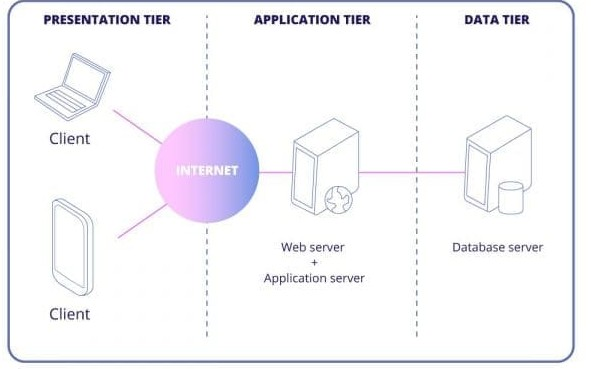
\includegraphics[width=0.7\textwidth]{3-tier-architecture}
    \end{center}
    \caption{The three-tier architecture}
  \end{figure}
\end{frame}

\note{
  GecWeb using the three-tier architecture, also known as the Model-View-Controller (MVC) architecture.

  Three-tier architecture is a well-known software application architecture that organizes applications into three logical and physical tiers: the presentation tier, or user interface; the application tier, where data is processed; and the data tier, where application data is stored and managed.
}

\begin{frame}{Architecture design}
  \begin{figure}
    \begin{center}
      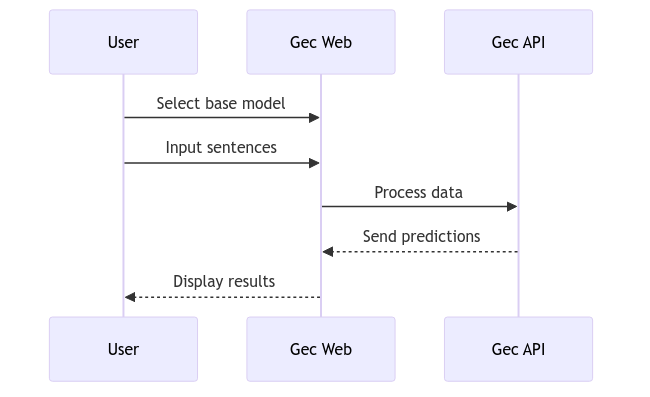
\includegraphics[width=0.7\textwidth]{usecase1}
    \end{center}
    \caption{Sequence Diagram of GecWeb}
  \end{figure}
\end{frame}

\note{
  Apply this architecture to GecWeb, we have:

  The presentation layer, or the user interface.
  For this layer, I use Flask and Bootstrap framework.
  It is responsible for rendering the input text box, output text box, and correction highlights.

  Next, the application Layer.
  For this layer, I use Flask RESTful API.
  This layer is responsible for handling user requests, managing the selection of GEC models and the system combination methods.

  Finally, the data Layer.
  Although no database is used in GecWeb, the GEC models are still considered part of the data layer.
  It handles the interaction with the underlying GEC systems.
  It takes the input text from the application layer, run it through the selected GEC models, and return the
  corrected sentences to the application layer.
}

\subsection{Process flow}

\begin{frame}{Process flow}
  \begin{figure}
    \begin{center}
      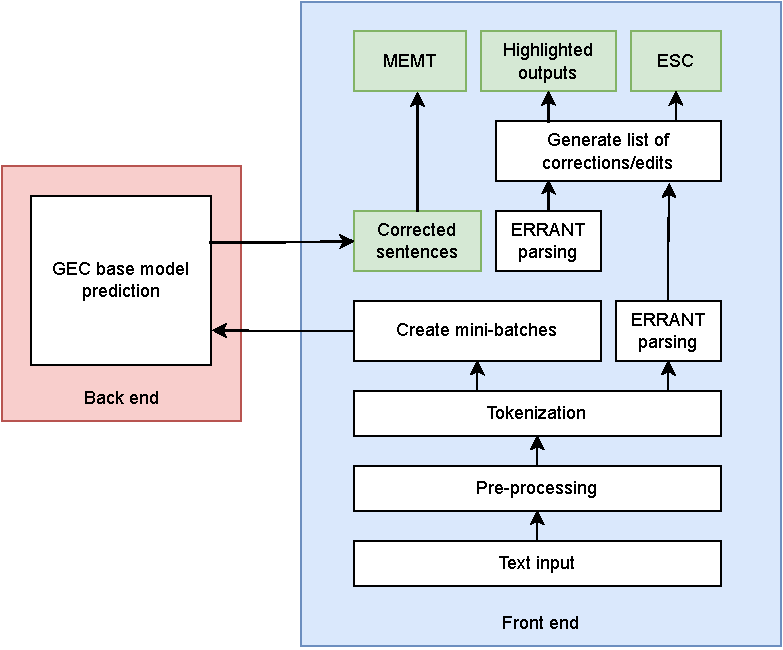
\includegraphics[height=0.7\textheight]{flowchart}
    \end{center}
    \caption{The process flow of GecWeb}
  \end{figure}
\end{frame}

\note{
  Now let's take a look at the process flow of GecWeb.

  All inputs are first split by line and segmented into sentences.
  The line index for each sentence is recorded to retain the text structure in the output.
  Then, the web interface tokenizes the sentences and combines them into mini-batches to be sent to the base models' API.
  If the user chooses to highlight the corrections or combine multiple base models with ESC, the web interface will also use ERRANT to parse the input sentences.
  After receiving the output sentences from each base model, the interface will then parse the base models and outputs using ERRANT if the user chooses to highlight corrections or use ESC.
  If not, the outputs are sent to MEMT if the user chooses to combine the models with MEMT.
  Otherwise, the output sentences are directly detokenized.
  Detokenization also applies to the combination method's output if the user selects more than one base model.
}
